\chapter*{Appendices} \\ % Use \chapter* to create an unnumbered chapter for appendices

\begin{figure}[h]
    \centering
    
\includegraphics[width=0.8\linewidth]{Cells 1 and 2.jpg}
    \caption{Appendix A}
    \label{fig:appendix_image_a}
\end{figure}

\begin{figure}[h]
    \centering
    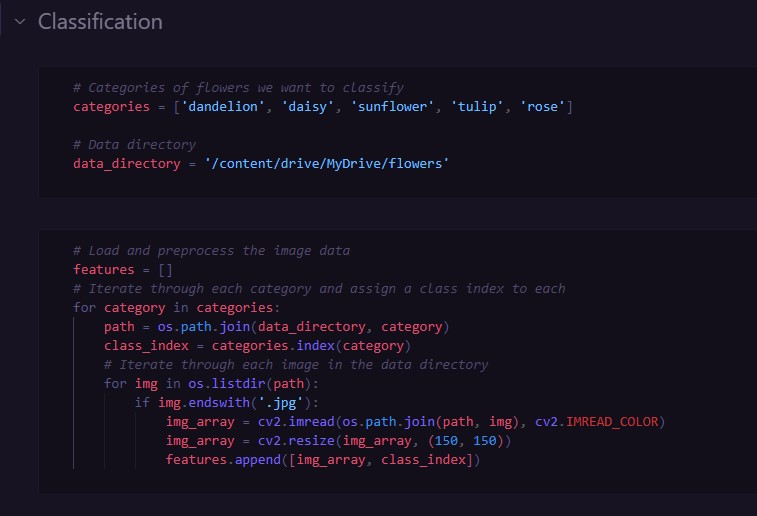
\includegraphics[width=0.8\linewidth]{Cells 3 and 4.jpg}
    \caption{Appendix B}
    \label{fig:appendix_image}
\end{figure}

\begin{figure}[h]
    \centering
    
\includegraphics[width=0.8\linewidth]{Cells image3.jpg}
    \caption{Appendix C}
    \label{fig:appendix_image}
\end{figure}


\begin{figure}[h]
    \centering
    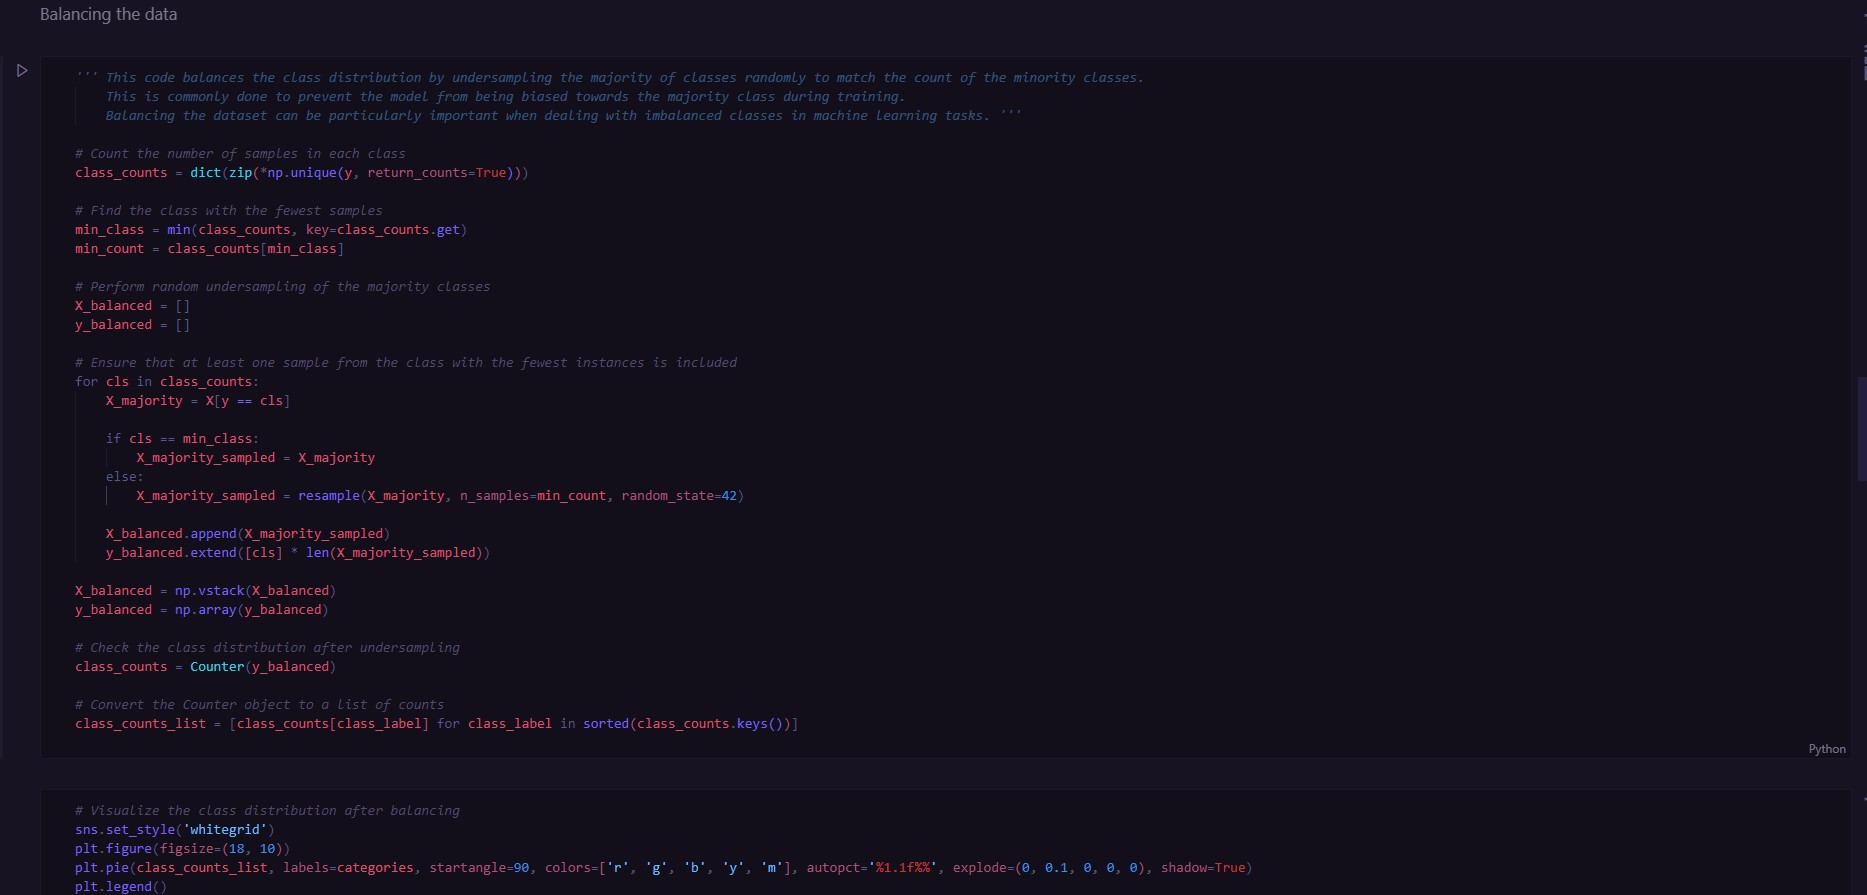
\includegraphics[width=0.8\linewidth]{cells image 4.jpg}
    \caption{Appendix D}
    \label{fig:appendix_image}
\end{figure}


\begin{figure}[h]
    \centering
    
\includegraphics[width=0.8\linewidth]{cells image 5.jpg}
    \caption{Appendix E}
    \label{fig:appendix_image}
\end{figure}


\begin{figure}[h]
    \centering
    
\includegraphics[width=0.8\linewidth]{cells image 6.jpg}
    \caption{Appendix F}
    \label{fig:appendix_image}
\end{figure}


\begin{figure}[h]
    \centering
    
\includegraphics[width=0.8\linewidth]{cells image 7.jpg}
    \caption{Appendix G}
    \label{fig:appendix_image}
\end{figure}
